\documentclass[12pt]{article}

\usepackage[a4paper, margin=1in]{geometry}
\usepackage{hyperref}
\usepackage{enumitem}
\usepackage{graphicx}
\usepackage[table,xcdraw]{xcolor}

\title{OMNeT++ Fuzzy IP Scheduler\\\large{Overview, implementation, and analysis}}
\date{2021\\March}
\author{\\Tomas-Adrian Boboi\\Universitatea Politehnica Timișoara}

\begin{document}
    \maketitle
    \pagebreak
    
    \tableofcontents
    \pagebreak
    
    \section{Original assignment requirements}
        \subsection*{The simulation model}
            The simulation model consists of the following OMNeT++ modules:
            \begin{enumerate}
                \item{A number of mobile users. In the first stages of the model you can implement two identical users, then you can consider a number of K users, organized as an array of users. Each user generates IP packets according to a certain pattern: e.g. an IP packet at certain (random) time intervals, or a user generates files, a file consisting on a (random) number of IP packets. At the beginning the IP packets can be considered of fixed length, i.e. one IP packet = 1500 bytes. A user has a certain priority. There can be for example 3 or 4 priority levels. For 3 priority levels, they are (in increasing order): LP (low priority), medium priority (MP) and HP (high priority). For 4 levels, they are: non real-time (nrt) low priority and nrt HP, real-time (rt) LP and rt HP.}
                \item{A scheduler. The scheduler is situated in the same Omnet module as the queues. The queues are not per user, but per priority class. This means that the packets arriving from LP user will be stored in the LP queue, the packets from MP and respectively HP users will be stored in the MP and respectively HP queue. The scheduler reads the lengths of the queues and implements a scheduling algorithm that determines which queue will send data. The sending of a packet takes a time equal to its length divided by the line rate (i.e. 1500 bytes / 1 Mega bit per second). The scheduler cannot send another packet during this time interval.}
                \item{A sink. The sink models the destination of the data. When the data (i.e. IP) packets created by an user arrive to the sink module, the sink simply deletes the OMNeT++ messages representing the data packets. Also, the sink is used to collect statistics about the simulation, statistics that can be for each user, for each group of users (e.g. Low, Medium and High priority users) and/or for the entire system. These statistical information can be: the number of data packets that arrive to the sink, the mean, minimum and maximum delay of the data packets, etc.}
            \end{enumerate}
            In the OMNeT directories there is one called "samples", with different simulation models implemented in OMNeT++. From these samples, you can use as a starting point for your model the sources from the "fifo" system.
        
        \subsection*{Basic/minimal requirements}
            Implement the simulation model described above. The scheduling algorithm is not very important in this stage, it can be a simple round robin: each nonempty queue sends a data packet. Or it can be a priority queueing algorithm: a queue is not served until there are non-empty higher priority queues.

        \subsection*{For exam, there are two alternatives to improve the project}
            Implement one of the following scheduling algorithms:
            \begin{itemize}
                \item{Priority queueing (a lower priority queue is served if and only if all higher priority queues are empty)}
                \item{A weighted round robin: an action takes place every time when there are resources available. The winner of the action will be served. The criteria for the action is, firstly, the time elapsed since the user was served last time. Then, we can improve the algorithm by introducing weights (positive numbers >1). The time elapsed since the user was served last time is multiplied with user's weight. Then, a user with a higher weight will be served more often. Compare the performance (i.e. average delay, minimum and maximum delay) of the implemented algorithms.}
            \end{itemize}
    
        \subsection*{New requirements (addition of the \textit{fuzzy logic controller})}
            Use a fuzzy logic controller in order to adjust the weight of HP users (W\_HP) such that their average delay will be most of the time smaller than a certain value.
            
            If the scheduling algorithm is priority queueing (PQ), then we cannot apply fuzzy weight adaptation like above, since PQ does not use weights!

    \section{Network structure}
    The network is described by the \verb|IpScheduler.ned| file, which contains the users, which generate the IP packets, the packet handler, which handles the packets received from the users, and the sink, which receives the packets sent from the packet handler.

        \subsection{IpScheduler}
            \verb|IpScheduler| is the main network, where all the sub-components reside.
            \begin{figure}[htbp!]
                \centering
                \includegraphics[width=0.8\textwidth]{images/ip_scheduler.png}
                \caption{The main network structure}
            \end{figure}
        
        \subsection{PacketHandler}
            \verb|PacketHandler| is the component responsible with receiving the packets from the users, storing them in the corresponding queue, depending on the priority level of the users, scheduling the sending of the packets, and sending the packets to the sink.
            \begin{figure}[htbp!]
                \centering
                \includegraphics[width=0.45\textwidth]{images/packet_handler.png}
                \caption{The packet handler structure}
            \end{figure}
        
        \subsection{User}
            The \verb|User| is the component which generates IP packets at a certain rate, and sends them to be handled bu the \verb|PacketHandler|. The users are grouped in priority classes:
            \begin{itemize}
                \item{non-real-time, low priority (nrtLp)}
                \item{non-real-time, low priority (nrtHp)}
                \item{real-time, high priority (rtLp)}
                \item{real-time, low priority (rtHp)}
            \end{itemize}
            The size of the generated IP packets, the packet generation rate, and the number of users in each priority class can be configured in the \verb|ipsched/config/users.ini| and \verb|ipsched/config/user_packets.ini| files.

        \subsection{Queue}
            The \verb|Queue| is the module which stores the IP packets generated by the users, and sends them towards the sink, whenever the scheduler allows it. There are four queues, one for each priority class, and they all communicate with the scheduler bidirectionally: they receive control messages from the scheduler, and send packets to the scheduler, when asked to.
            The \textit{Queue} class contains a \verb|cPacketQueue| attribute, where the IP packets are stored.
            The \verb|Queue| module is also responsible with logging each queue's length, so we can collect data about the length of each queue at any given time.
        
        \subsection{Sink}
            The \verb|Sink| is a module whose only purpose is to receive the IP packets, delete them, and record statistics about them (packet lifetime, total number of packets, etc.).

        \subsection{Scheduler}
            The \verb|Scheduler| can be considered the most complex module of the system, and the most important, because it is responsible for deciding which queue sends a packet towards the sink. This job can be accomplished in multiple ways, and the current project provides two scheduler implementations: Weighted Round Robin, with and without the addition of the \textit{fuzzy logic controller}.

    \section{The fuzzy logic controller}
        \begin{figure}[!h]
            \centering
            \includegraphics[width=0.4\textwidth]{images/flc.png}
            \caption{The structure of the Fuzzy Logic Controller: the actual module, and the clock generator, which triggers its activation via messages}
        \end{figure}
        
        \subsection{The \textit{FLC\_gen} module}
            The \verb|Fuzzy Logic Controller Generator| module is a relatively simple module whose only purpose is to trigger the activation of the main \verb|Fuzzy Logic Controller| module, at a rate specified by the parameter \verb|flc_time|. Every \verb|flc_time| time intervals, a message is sent to the \verb|Fuzzy Logic Controller| module, which activates the latter and triggers the adjustment of the weight of the high-priority real-time users.
        
        \subsection{The \textit{FLC} module}
            The \verb|Fuzzy Logic Controller| module is responsible with adjusting the weight of the high-priority real-time users, so that their average delay stays within a given margin. It is activated at regular intervals, when it receives an activation message from the \verb|Fuzzy Logic Controller Generator| module.

            As a C++ class, in contains methods for fuzzyfying, defuzzyfying and scaling variables, with additional helper attributes to achieve the functionalities of these methods. Apart from these methods, the \verb|Fuzzy Logic Controller| module contains a method which performs fuzzy inference on a variable, and returns the result as an integer. We use this method with the current weight and the difference between the current delay and the desired delay as inputs, and as a result we get the change in weight that we need to apply to the current weight.

            We add this change in weight to our current weight to get the new one, which, hopefully, will bring the average packet delay of the high-priority real-time users down towards the desired delay, and then maintain it.

            Of course, this whole process happens when the \verb|Fuzzy Logic Controller| module is activated by a message from the \verb|Fuzzy Logic Controller Generator| module, and so the rate at which the generator sends activation messages has an impact on the average delay variations.
    
    \section{Experiments}
        \subsection{Simulation parameters}
            In this project, I shall choose the following parameters to vary and study their effects:
            \begin{itemize}
                \item{the packet generation rate $r_{gen}$, that is, the rate at which each user generates IP packets and sends them towards the \verb|Sink| module through the \verb|Scheduler|; the packets are generated following an exponential distribution with mean $r_{gen}$}
                \item{the wanted delay $w_d$, that is, the average packet delay that we want to achieve for our high-priority real-time users}
                \item{the \verb|Fuzzy Logic Controller| module activation rate $r_{a}$, that is, the rate at which the \verb|Fuzzy Logic Controller Generator| module sends activation messages to the FLC to trigger its function}
                \item{the number of users in each class $n_{nrtLp}, n_{nrtHp}, n_{rtLp}, n_{rtHp}$}
            \end{itemize}

            For each experiment that will follow, I shall present a table showing the values of the previously mentioned parameters.

            The metric that is being evaluated is the average packet delay, that is, the average time it takes for the packet to reach the \verb|Sink| module, after being generated by the users. The average is taken over all previous packets, over the entire simulation time. The simulation time is capped at 1 second, therefore this mertric will tell us the expected packet delay after 1 second of network utilization.

            For all upcoming experiments, the horizontal axis (representing the simulation time) will be measured in seconds, and the vertical axis (representing the average packet delay) will be measured in microseconds.

            The color coding of the graphs will be the same for all experiments:
            \begin{itemize}
                \item{the {\color{green}{green}} line represents the average delay of the non-real-time low-priority users}
                \item{the {\color{red}{red}} line represents the average delay of the non-real-time high-priority users}
                \item{the {\color{blue}{blue}} line represents the average delay of the real-time low-priority users}
                \item{the {\color{orange}{orange}} line represents the average delay of the real-time high-priority users}
            \end{itemize}

            In addition, the initial weights of the users are 1, 2, 4, and 8, for non-real-time low-priority, non-real-time high-priority, real-time low-priority, and real-time high-priority, respectively.
        
        \pagebreak
        \subsection{Standalone experiments}
            \subsection{Varying the packet generation rate $r_{gen}$}
                \subsubsection{Experiment \#1}
                    \begin{table}[!h]
                        \centering
                        \begin{tabular}{|c|c|c|cccc|}
                            \hline
                            $r_{gen} [us]$ & $w_{d} [us]$ & $r_{a} [us]$ & $n_{nrtLp}$ & $n_{nrtHp}$ & $n_{rtLp}$ & $n_{rtHp}$ \\ \hline
                            1000           & 50000         & 1000         & 20        & 20        & 20       & 20       \\ \hline
                        \end{tabular}
                    \end{table}

                    \begin{figure}[!h]
                        \centering
                        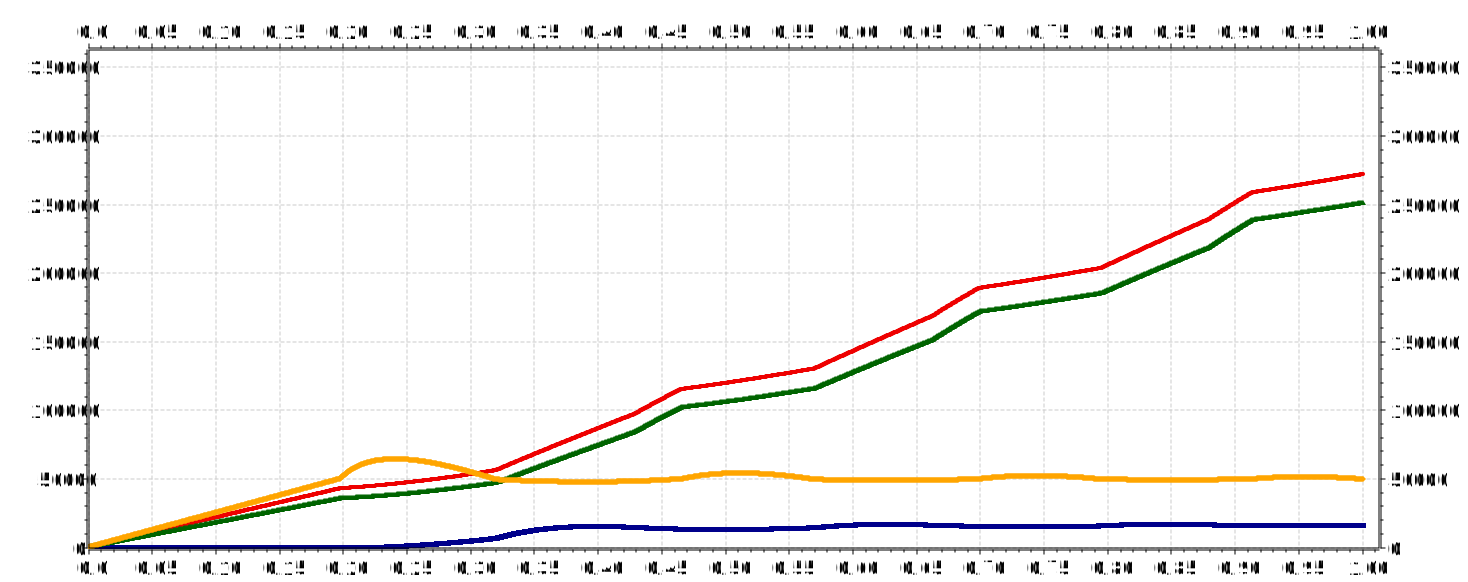
\includegraphics[width=\textwidth]{images/exp_001.png}
                        \caption{Here we see the FLC in action. When the average delay is under $w_{d}$, the FLC has no effect, but after the delay crosses the threshold, the FLC kicks in and adjusts the weights, bringing the average delay to the desired value.}
                    \end{figure}

                \pagebreak
                \subsubsection{Experiment \#2}
                    \begin{table}[!h]
                        \centering
                        \begin{tabular}{|c|c|c|cccc|}
                            \hline
                            $r_{gen} [us]$ & $w_{d} [us]$ & $r_{a} [us]$ & $n_{nrtLp}$ & $n_{nrtHp}$ & $n_{rtLp}$ & $n_{rtHp}$ \\ \hline
                            750           & 50000         & 1000         & 20        & 20        & 20       & 20       \\ \hline
                        \end{tabular}
                    \end{table}

                    \begin{figure}[!h]
                        \centering
                        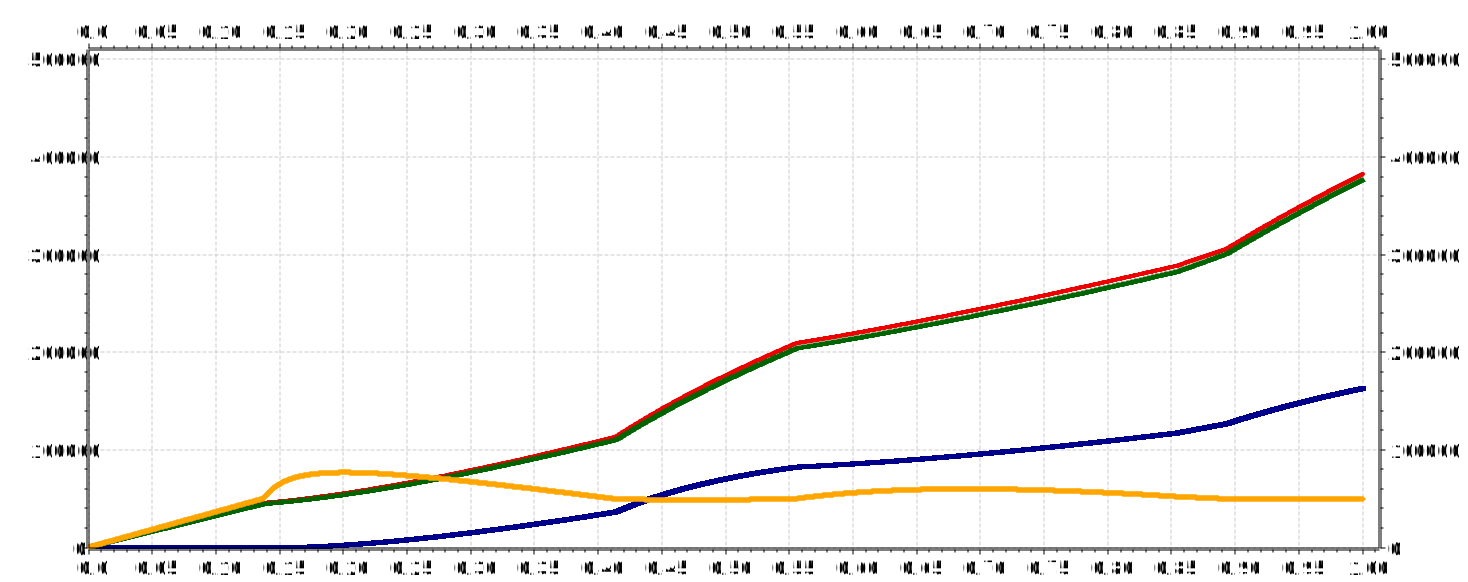
\includegraphics[width=\textwidth]{images/exp_002.png}
                        \caption{We notice the same phenomena as before, except this time the network is under more load, and it takes a little more time for the average delay to stabilize at the desired value.}
                    \end{figure}

                \subsubsection{Experiment \#3}
                    \begin{table}[!h]
                        \centering
                        \begin{tabular}{|c|c|c|cccc|}
                            \hline
                            $r_{gen} [us]$ & $w_{d} [us]$ & $r_{a} [us]$ & $n_{nrtLp}$ & $n_{nrtHp}$ & $n_{rtLp}$ & $n_{rtHp}$ \\ \hline
                            500           & 50000         & 1000         & 20        & 20        & 20       & 20       \\ \hline
                        \end{tabular}
                    \end{table}

                    \begin{figure}[!h]
                        \centering
                        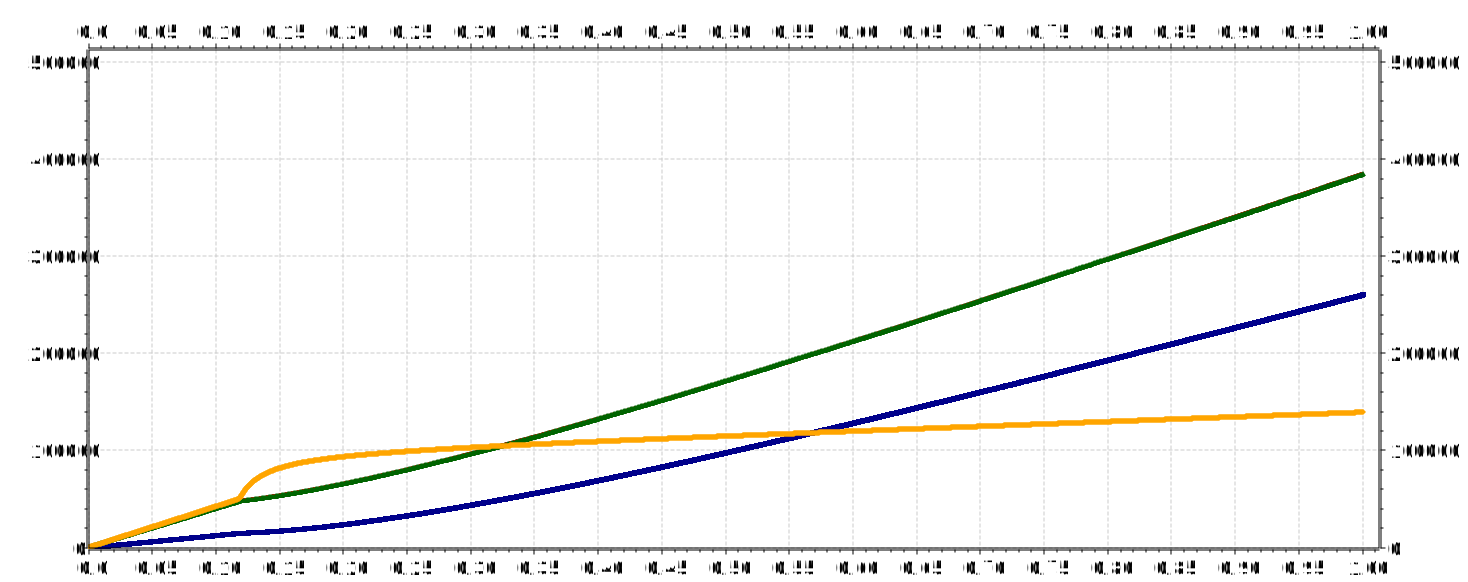
\includegraphics[width=\textwidth]{images/exp_003.png}
                        \caption{Here, the network is at full capacity. The FLC tries to improve the average delay, but fails, and the delays for all users start growing out of control.}
                    \end{figure}

            \subsection{Varying the wanted delay $w_{d}$}
                \subsubsection{Experiment \#4}
                    \begin{table}[!h]
                        \centering
                        \begin{tabular}{|c|c|c|cccc|}
                            \hline
                            $r_{gen} [us]$ & $w_{d} [us]$ & $r_{a} [us]$ & $n_{nrtLp}$ & $n_{nrtHp}$ & $n_{rtLp}$ & $n_{rtHp}$ \\ \hline
                            750           & 100000         & 1000         & 20        & 20        & 20       & 20       \\ \hline
                        \end{tabular}
                    \end{table}

                    \begin{figure}[!h]
                        \centering
                        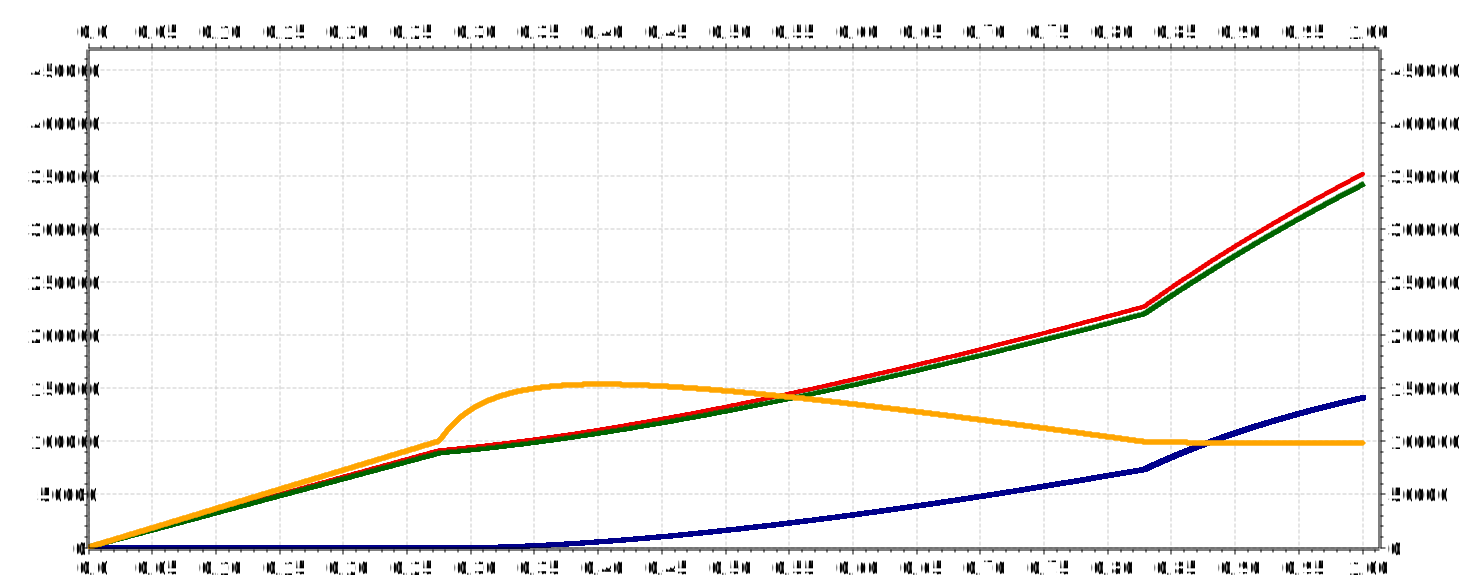
\includegraphics[width=\textwidth]{images/exp_004.png}
                        \caption{The FLC causes the average delay to converge, after an initial overshoot, to the desired value}
                    \end{figure}

                \subsubsection{Experiment \#5}
                    \begin{table}[!h]
                        \centering
                        \begin{tabular}{|c|c|c|cccc|}
                            \hline
                            $r_{gen} [us]$ & $w_{d} [us]$ & $r_{a} [us]$ & $n_{nrtLp}$ & $n_{nrtHp}$ & $n_{rtLp}$ & $n_{rtHp}$ \\ \hline
                            750           & 50000         & 1000         & 20        & 20        & 20       & 20       \\ \hline
                        \end{tabular}
                    \end{table}

                    \begin{figure}[!h]
                        \centering
                        \includegraphics[width=\textwidth]{images/exp_005.png}
                        \caption{Decreasing the desired average delay also decreases the convergence time and the initial overshoot, and so the average delay settles a little faster}
                    \end{figure}
                    \pagebreak

                \subsubsection{Experiment \#6}
                    \begin{table}[!h]
                        \centering
                        \begin{tabular}{|c|c|c|cccc|}
                            \hline
                            $r_{gen} [us]$ & $w_{d} [us]$ & $r_{a} [us]$ & $n_{nrtLp}$ & $n_{nrtHp}$ & $n_{rtLp}$ & $n_{rtHp}$ \\ \hline
                            750           & 5000         & 1000         & 20        & 20        & 20       & 20       \\ \hline
                        \end{tabular}
                    \end{table}

                    \begin{figure}[!h]
                        \centering
                        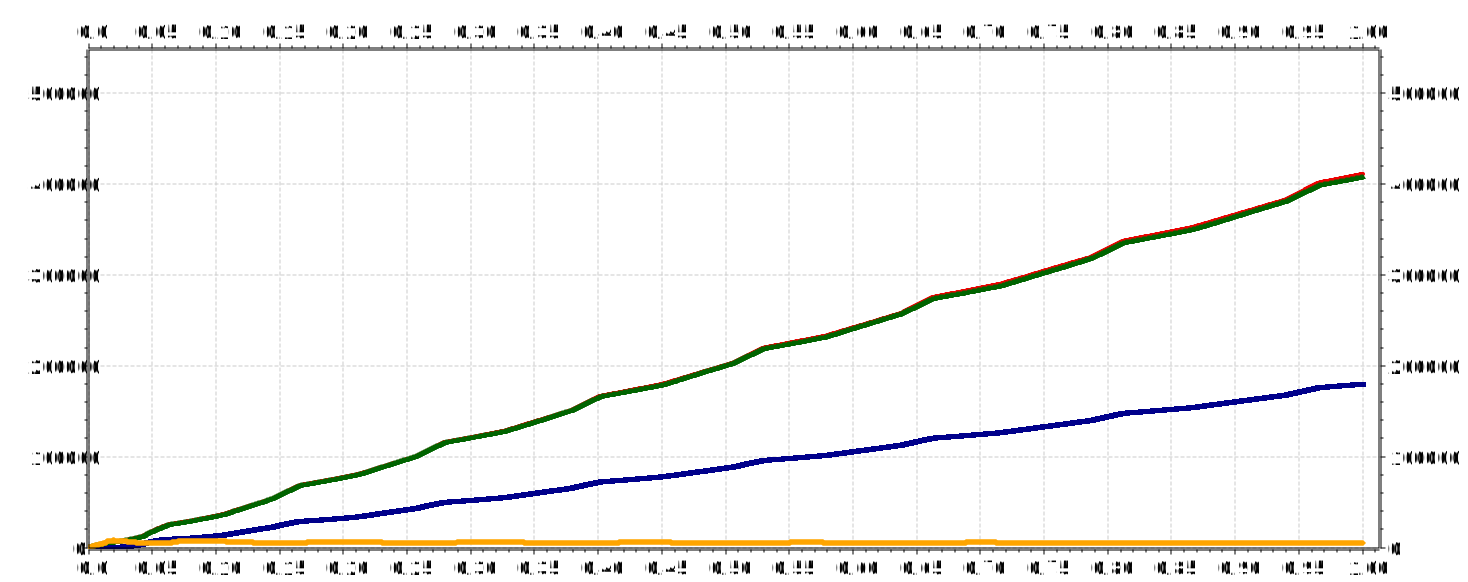
\includegraphics[width=\textwidth]{images/exp_006.png}
                        \caption{Decreasing the average delay even further leads to even faster convergence, at the expense, of course, of the other user's delays, which have gone up significantly}
                    \end{figure}
            \pagebreak

            \subsection{Varying the FLC activation rate $r_{a}$}
                \subsubsection{Experiment \#7}
                    \begin{table}[!h]
                        \centering
                        \begin{tabular}{|c|c|c|cccc|}
                            \hline
                            $r_{gen} [us]$ & $w_{d} [us]$ & $r_{a} [us]$ & $n_{nrtLp}$ & $n_{nrtHp}$ & $n_{rtLp}$ & $n_{rtHp}$ \\ \hline
                            750           & 50000         & 250000         & 20        & 20        & 20       & 20       \\ \hline
                        \end{tabular}
                    \end{table}

                    \begin{figure}[!h]
                        \centering
                        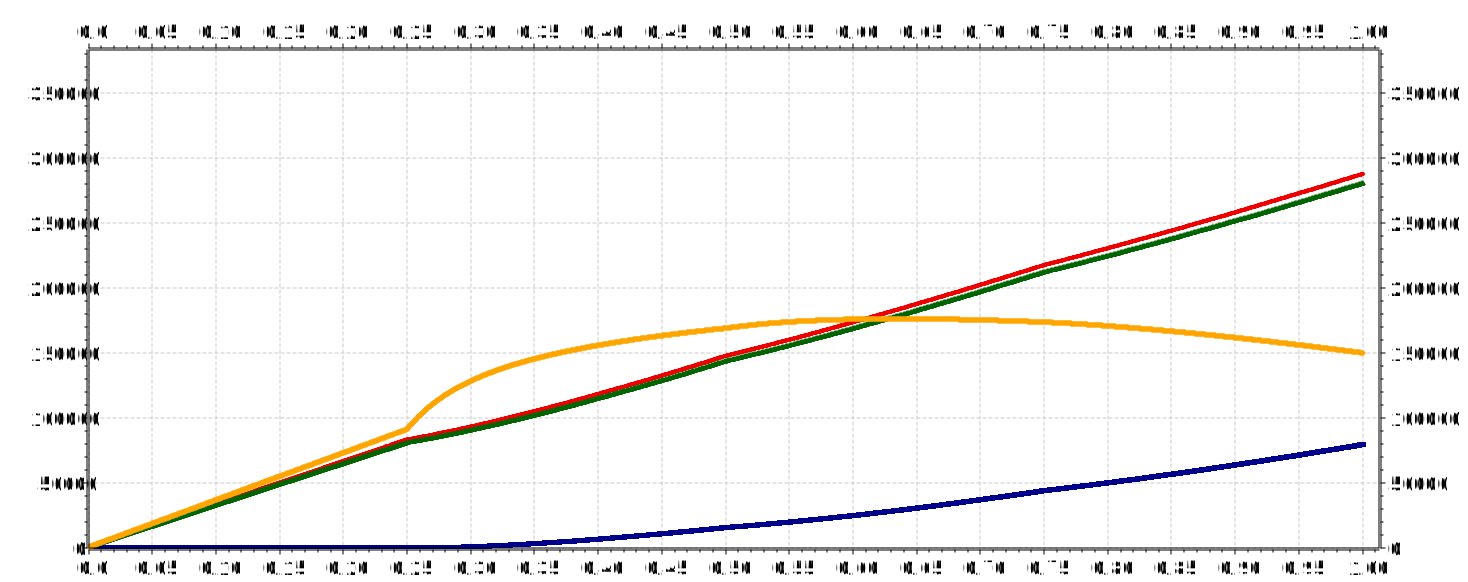
\includegraphics[width=\textwidth]{images/exp_007.png}
                        \caption{In this case, the activation time is way too low for the FLC to be able to take action, and so the average delay doesn't get to stabilize at the desired value. Leaving the simulation run for more time would eventually lead to the average delay stabilizing.}
                    \end{figure}

                \subsubsection{Experiment \#8}
                    \begin{table}[!h]
                        \centering
                        \begin{tabular}{|c|c|c|cccc|}
                            \hline
                            $r_{gen} [us]$ & $w_{d} [us]$ & $r_{a} [us]$ & $n_{nrtLp}$ & $n_{nrtHp}$ & $n_{rtLp}$ & $n_{rtHp}$ \\ \hline
                            750           & 50000         & 75000         & 20        & 20        & 20       & 20       \\ \hline
                        \end{tabular}
                    \end{table}

                    \begin{figure}[!h]
                        \centering
                        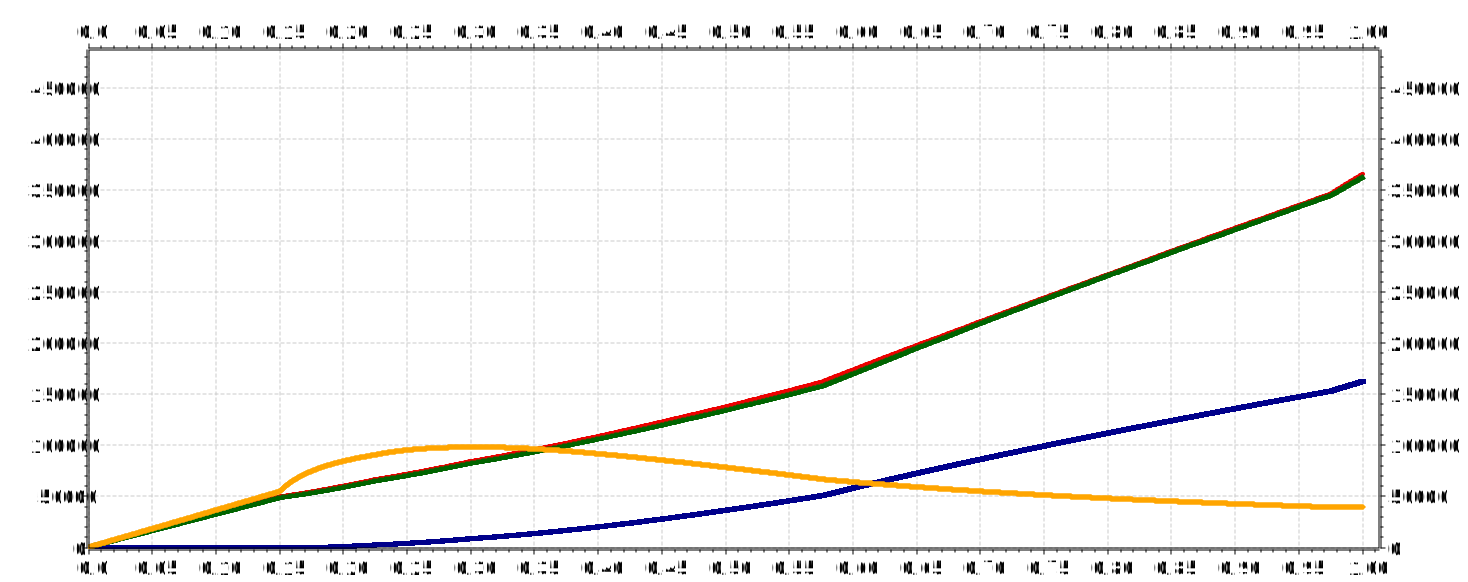
\includegraphics[width=\textwidth]{images/exp_008.png}
                        \caption{Here, the convergence time is decreased, due to the FLC adjusting the weights more often, but the average delay still fluctuates a little after one second.}
                    \end{figure}

                \subsubsection{Experiment \#9}
                    \begin{table}[!h]
                        \centering
                        \begin{tabular}{|c|c|c|cccc|}
                            \hline
                            $r_{gen} [us]$ & $w_{d} [us]$ & $r_{a} [us]$ & $n_{nrtLp}$ & $n_{nrtHp}$ & $n_{rtLp}$ & $n_{rtHp}$ \\ \hline
                            750           & 50000         & 10000         & 20        & 20        & 20       & 20       \\ \hline
                        \end{tabular}
                    \end{table}

                    \begin{figure}[!h]
                        \centering
                        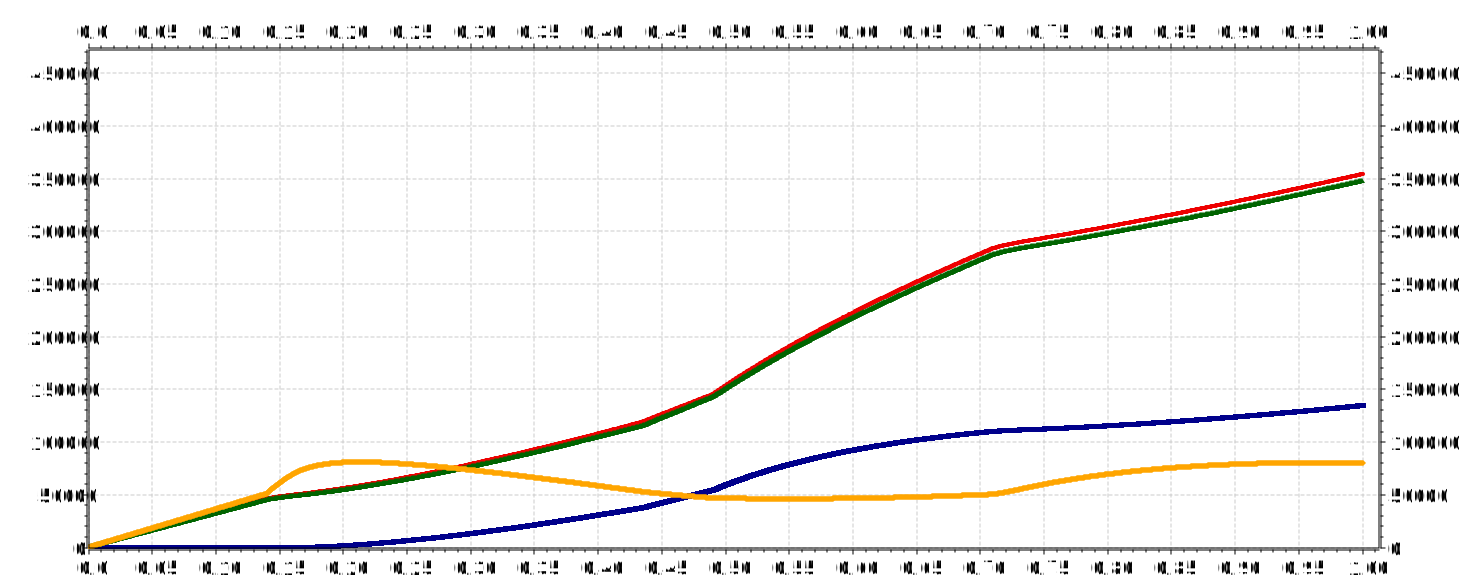
\includegraphics[width=\textwidth]{images/exp_009.png}
                        \caption{An anomaly can be seen here: even though the activation rate is lower than in the previous experiment, the average delay seems to converge less steadily, as the difference between the actual delay and the desired delay is larger.}
                    \end{figure}

                \subsubsection{Experiment \#10}
                    \begin{table}[!h]
                        \centering
                        \begin{tabular}{|c|c|c|cccc|}
                            \hline
                            $r_{gen} [us]$ & $w_{d} [us]$ & $r_{a} [us]$ & $n_{nrtLp}$ & $n_{nrtHp}$ & $n_{rtLp}$ & $n_{rtHp}$ \\ \hline
                            750           & 50000         & 1000         & 20        & 20        & 20       & 20       \\ \hline
                        \end{tabular}
                    \end{table}

                    \begin{figure}[!h]
                        \centering
                        \includegraphics[width=\textwidth]{images/exp_010.png}
                        \caption{This situation has been previously seen, and in this case the rate is sufficient to allow for the average delay to stabilize at the desired value before the one second has passed.}
                    \end{figure}

            \subsection{Varying the number of users in each priority class}
                \subsubsection{Experiments \#11, \#12, \#13, and \#14}
                    \begin{table}[!h]
                        \centering
                        \begin{tabular}{|c|c|c|cccc|}
                            \hline
                            $r_{gen} [us]$ & $w_{d} [us]$ & $r_{a} [us]$ & $n_{nrtLp}$ & $n_{nrtHp}$ & $n_{rtLp}$ & $n_{rtHp}$ \\ \hline
                            750           & 50000         & 1000         & 30        & 17        & 17       & 17       \\ \hline
                        \end{tabular}
                    \end{table}

                    \begin{figure}[!h]
                        \centering
                        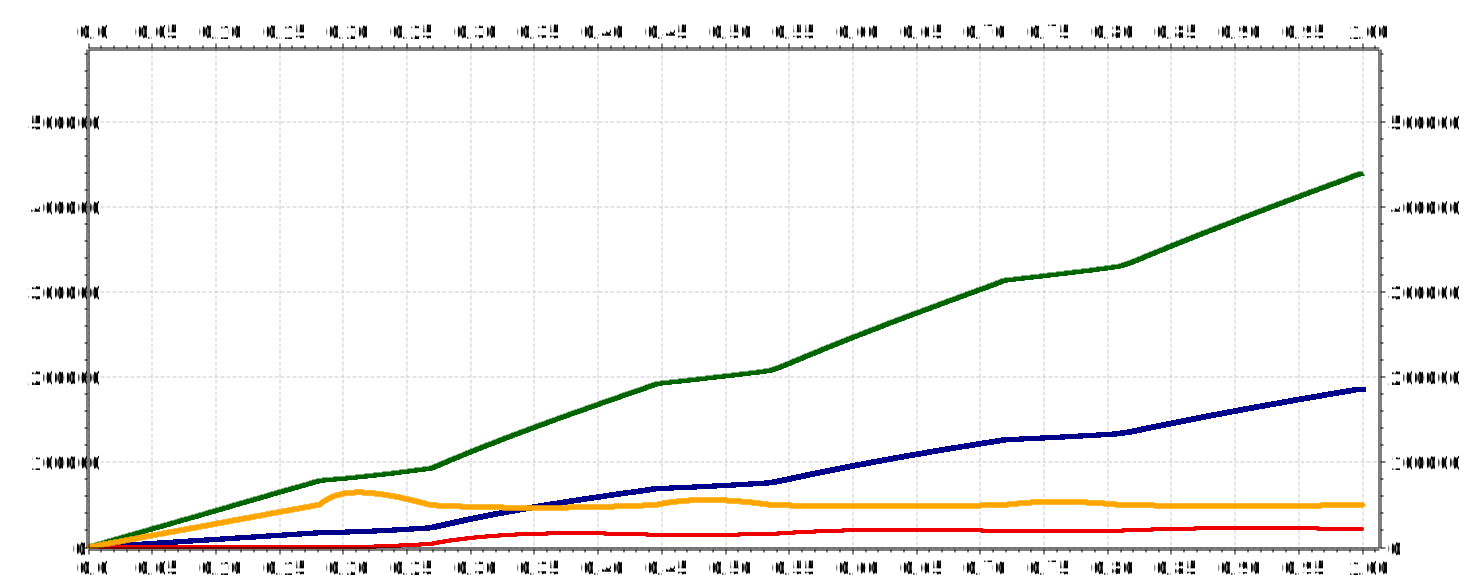
\includegraphics[width=\textwidth]{images/exp_011.png}
                        \caption{Experiment \#11 results}
                    \end{figure}

                    \begin{table}[!h]
                        \centering
                        \begin{tabular}{|c|c|c|cccc|}
                            \hline
                            $r_{gen} [us]$ & $w_{d} [us]$ & $r_{a} [us]$ & $n_{nrtLp}$ & $n_{nrtHp}$ & $n_{rtLp}$ & $n_{rtHp}$ \\ \hline
                            750           & 50000         & 1000         & 17        & 30        & 17       & 17       \\ \hline
                        \end{tabular}
                    \end{table}

                    \begin{figure}[!h]
                        \centering
                        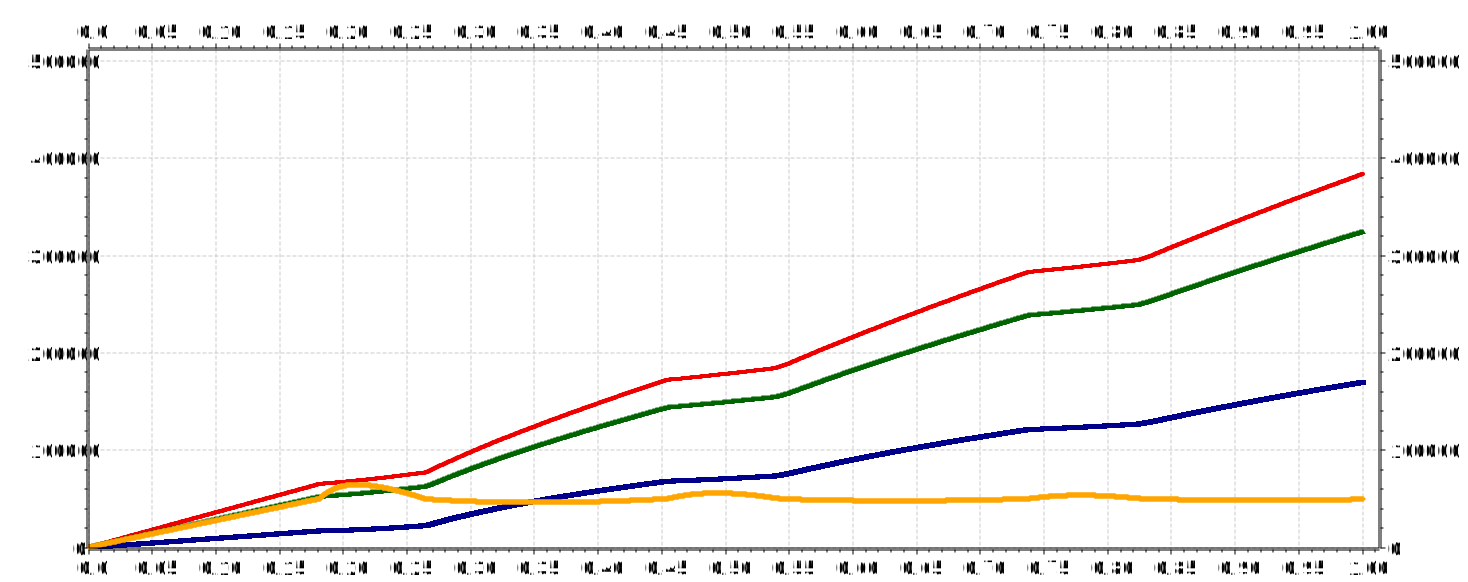
\includegraphics[width=\textwidth]{images/exp_012.png}
                        \caption{Experiment \#12 results}
                    \end{figure}
                    \pagebreak

                    \begin{table}[!h]
                        \centering
                        \begin{tabular}{|c|c|c|cccc|}
                            \hline
                            $r_{gen} [us]$ & $w_{d} [us]$ & $r_{a} [us]$ & $n_{nrtLp}$ & $n_{nrtHp}$ & $n_{rtLp}$ & $n_{rtHp}$ \\ \hline
                            750           & 50000         & 1000         & 17        & 17        & 30       & 17       \\ \hline
                        \end{tabular}
                    \end{table}

                    \begin{figure}[!h]
                        \centering
                        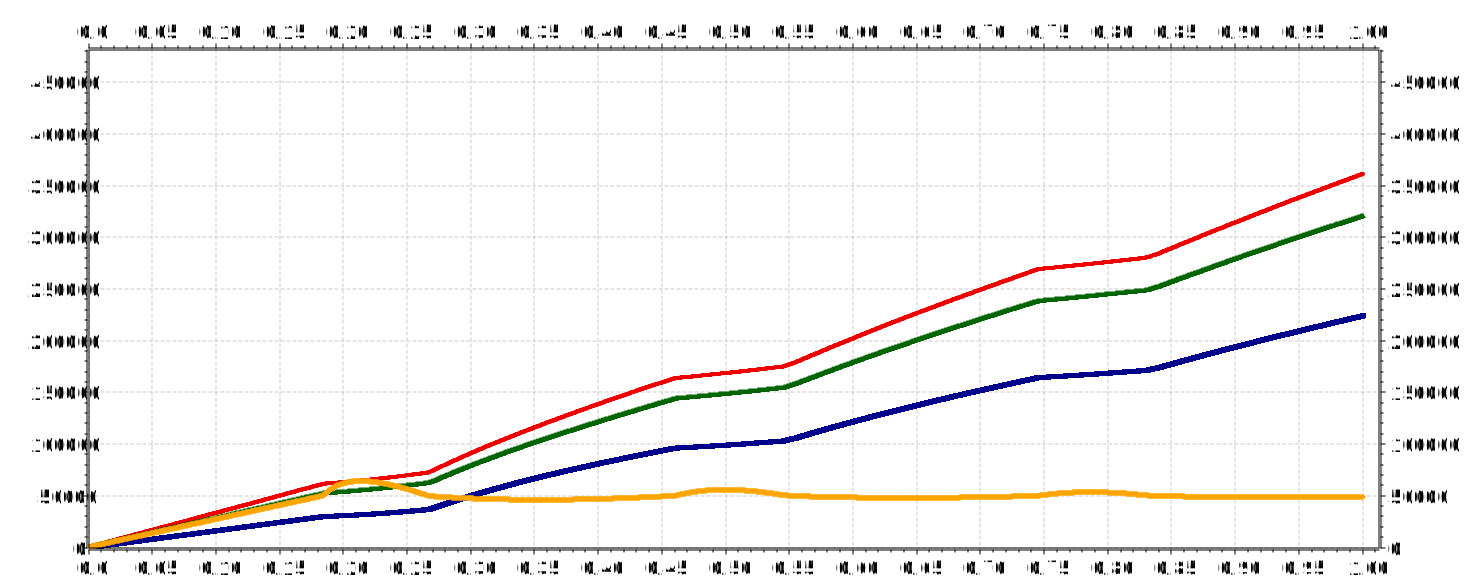
\includegraphics[width=\textwidth]{images/exp_013.png}
                        \caption{Experiment \#13 results}
                    \end{figure}

                    \begin{table}[!h]
                        \centering
                        \begin{tabular}{|c|c|c|cccc|}
                            \hline
                            $r_{gen} [us]$ & $w_{d} [us]$ & $r_{a} [us]$ & $n_{nrtLp}$ & $n_{nrtHp}$ & $n_{rtLp}$ & $n_{rtHp}$ \\ \hline
                            750           & 50000         & 1000         & 17        & 17        & 17       & 30       \\ \hline
                        \end{tabular}
                    \end{table}

                    \begin{figure}[!h]
                        \centering
                        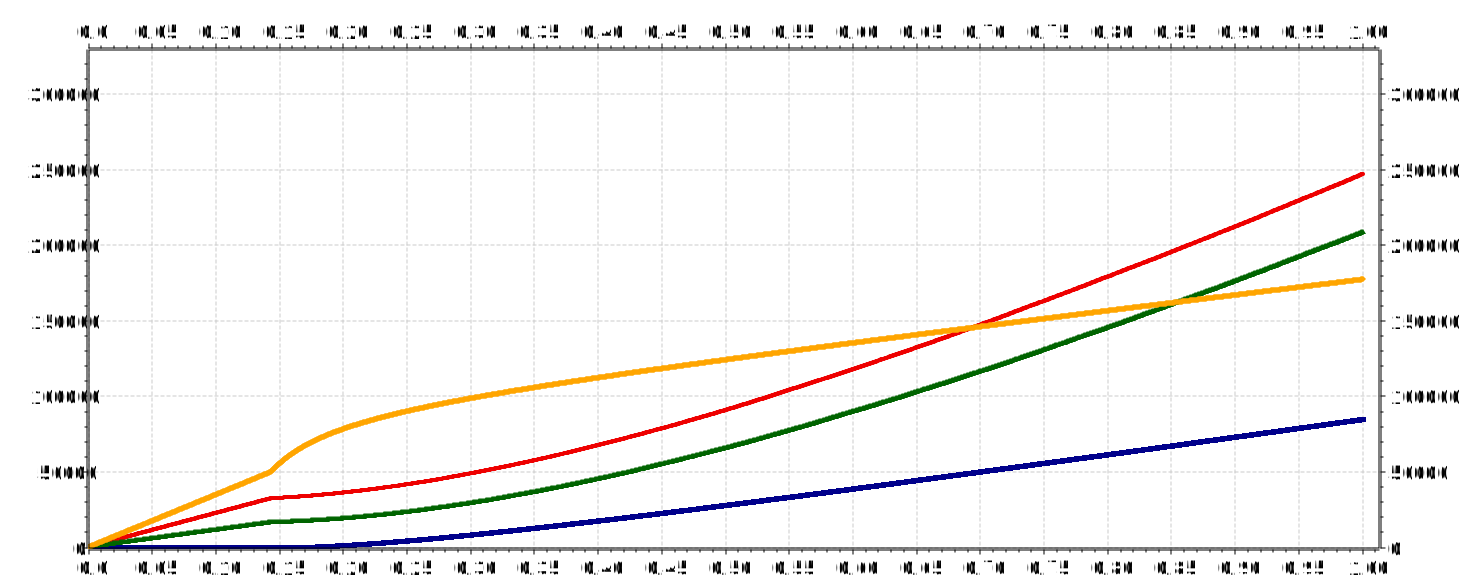
\includegraphics[width=\textwidth]{images/exp_014.png}
                        \caption{Experiment \#14 results}
                    \end{figure}

                    The conclusion of experiments \#11, \#12, and \#13 can be formualted as follows: the class with the highest number of users generally tends to have the highest average delay at the end of the simulationm,when taking into consideration the non-real-time classes. Experiment \#13 reveals that a higher number of real-time low-priority users does lead to a higher average delay than before, but it still is lower than that of the non-real-time classes. In all of these cases, though, the FLC manages to stabilize the average delay of the real-time high-priority users to the desired value.

                    Experiment \#14, however, tells a different story. Increasing the total number of real-time high-priority users leads to the FLC being overwhelmed, as it does no longer manage to bring the average delay to a steady value, but instead it grows out of control.
        
        \subsection{Comparative experiments}
            In this section, we shall do a comparison between our FLC-enhanced Weighted-Round-Robin-based scheduler, and a classic WRR scheduler, and see how the two implementations compare against each other. In order to do a fair comparison of the two, we shall first select and vary in our experiments those parameters that are common to the two implementations, namely the packet generation rate, and the number of users in each priority class.

            \subsubsection{Comparative experiment \#1: baseline testing}
                \begin{table}[!h]
                    \centering
                    \begin{tabular}{|c|c|c|cccc|}
                        \hline
                        $r_{gen} [us]$ & {\color[HTML]{9B9B9B} $w_{d} [us]$} & {\color[HTML]{9B9B9B} $r_{a} [us]$} & $n_{nrtLp}$ & $n_{nrtHp}$ & $n_{rtLp}$ & $n_{rtHp}$ \\ \hline
                        1000           & {\color[HTML]{9B9B9B} 50000}        & {\color[HTML]{9B9B9B} 1000}         & 20          & 20          & 20         & 20         \\ \hline
                    \end{tabular}
                \end{table}

                \begin{figure}[!h]
                    \centering
                    \includegraphics[width=\textwidth]{images/cexp_001_1.png}
                    \caption{FLC-enhanced scheduler results}
                \end{figure}

                \begin{figure}[!h]
                    \centering
                    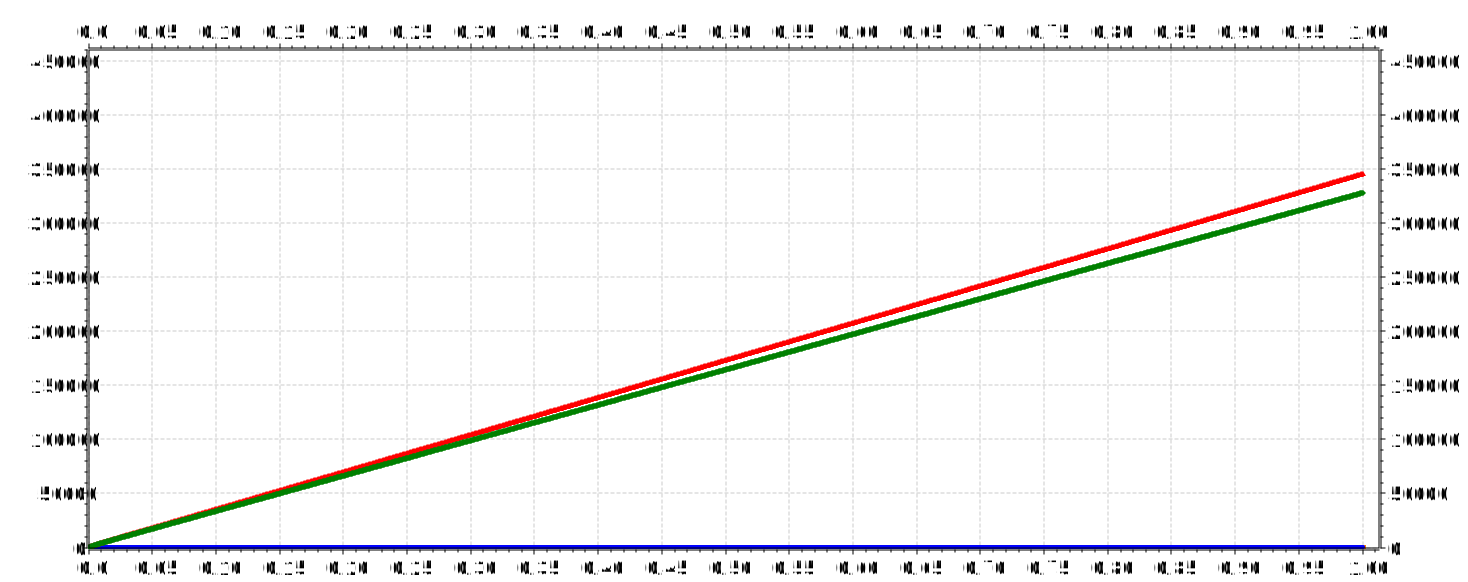
\includegraphics[width=\textwidth]{images/cexp_001_2.png}
                    \caption{Regular WRR scheduler results}
                \end{figure}
                \pagebreak

                In this experiment, even though the average delays of the real-time users are higher in the FLC-enhanced sceduler's case, we can see that the FLC leads to a more fair distribution of delays. Without the FLC, the delays of the non-real-time users go up faster than with the FLC.
                
                We notice a compromise in the FLC-enhanced case: the real-time user's average delays are slightly higher, while the non-real-time user's average delays are slightly lower.

                Had we set a lower desired average delay for the real-time high-priority users, the results would have been more similar.

            \subsubsection{Comparative experiment \#2: slightly higher network load}
                \begin{table}[!h]
                    \centering
                    \begin{tabular}{|c|c|c|cccc|}
                        \hline
                        $r_{gen} [us]$ & {\color[HTML]{9B9B9B} $w_{d} [us]$} & {\color[HTML]{9B9B9B} $r_{a} [us]$} & $n_{nrtLp}$ & $n_{nrtHp}$ & $n_{rtLp}$ & $n_{rtHp}$ \\ \hline
                        750           & {\color[HTML]{9B9B9B} 50000}        & {\color[HTML]{9B9B9B} 1000}         & 20          & 20          & 20         & 20         \\ \hline
                    \end{tabular}
                \end{table}

                \begin{figure}[!h]
                    \centering
                    \includegraphics[width=\textwidth]{images/cexp_002_1.png}
                    \caption{FLC-enhanced scheduler results}
                \end{figure}

                \begin{figure}[!h]
                    \centering
                    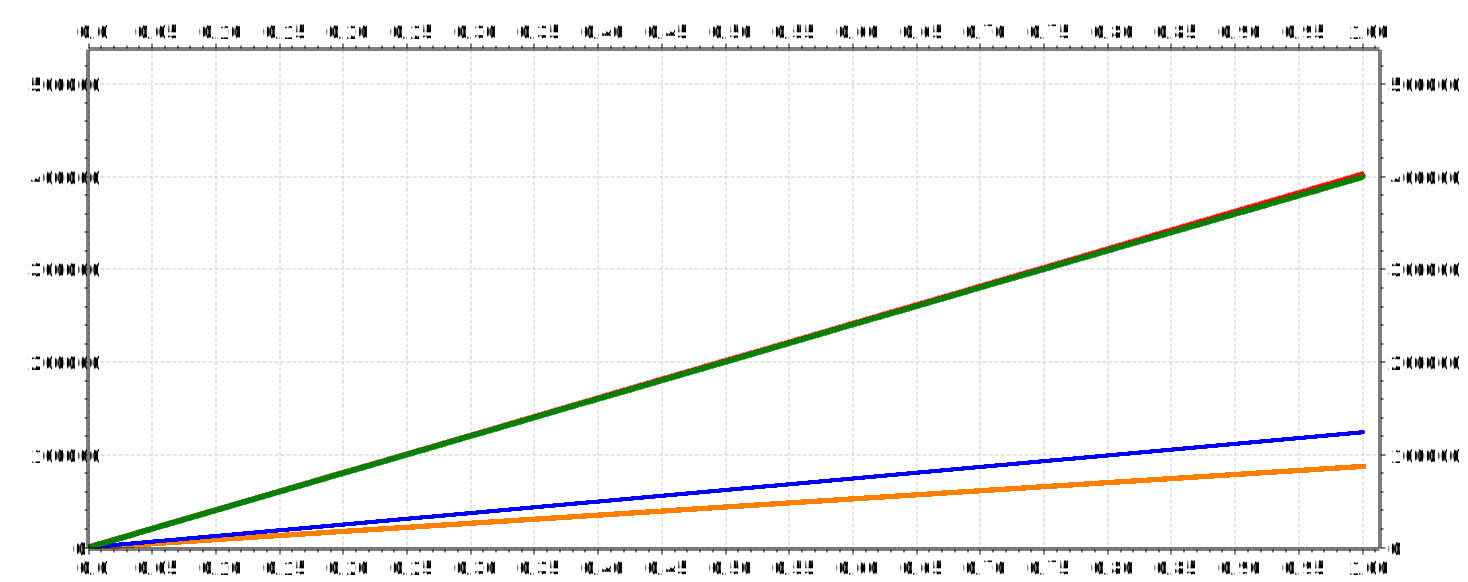
\includegraphics[width=\textwidth]{images/cexp_002_2.png}
                    \caption{Regular WRR scheduler results}
                \end{figure}
                \pagebreak

                In this scenario, in which the load is higher than previously, the FLC-enhanced scheduler proves its superiority. It manages to maintain the average delay of the real-time high-priority users at the desired level. The regular scheduler, on the other hand, has lost control, and the average delays are starting to grow steadily, without any signs of stopping.

                Therefore, we can conclude that in a situation in which the network load is higher, the FLC-enhanced scheduler is superior, at least when it comes to the real-time high-priority user's happiness (the other classes do not do so well). There is a sweet-spot for this behaviour, of course, as increasing the network load even further would lead to both implementations failing to maintain the average delays in accepatable ranges.

            \subsubsection{Comparative experiment \#3: more real-time high-priority users}
                \begin{table}[!h]
                    \centering
                    \begin{tabular}{|c|c|c|cccc|}
                        \hline
                        $r_{gen} [us]$ & {\color[HTML]{9B9B9B} $w_{d} [us]$} & {\color[HTML]{9B9B9B} $r_{a} [us]$} & $n_{nrtLp}$ & $n_{nrtHp}$ & $n_{rtLp}$ & $n_{rtHp}$ \\ \hline
                        1000           & {\color[HTML]{9B9B9B} 50000}        & {\color[HTML]{9B9B9B} 1000}         & 17          & 17          & 17         & 30         \\ \hline
                    \end{tabular}
                \end{table}

                \begin{figure}[!h]
                    \centering
                    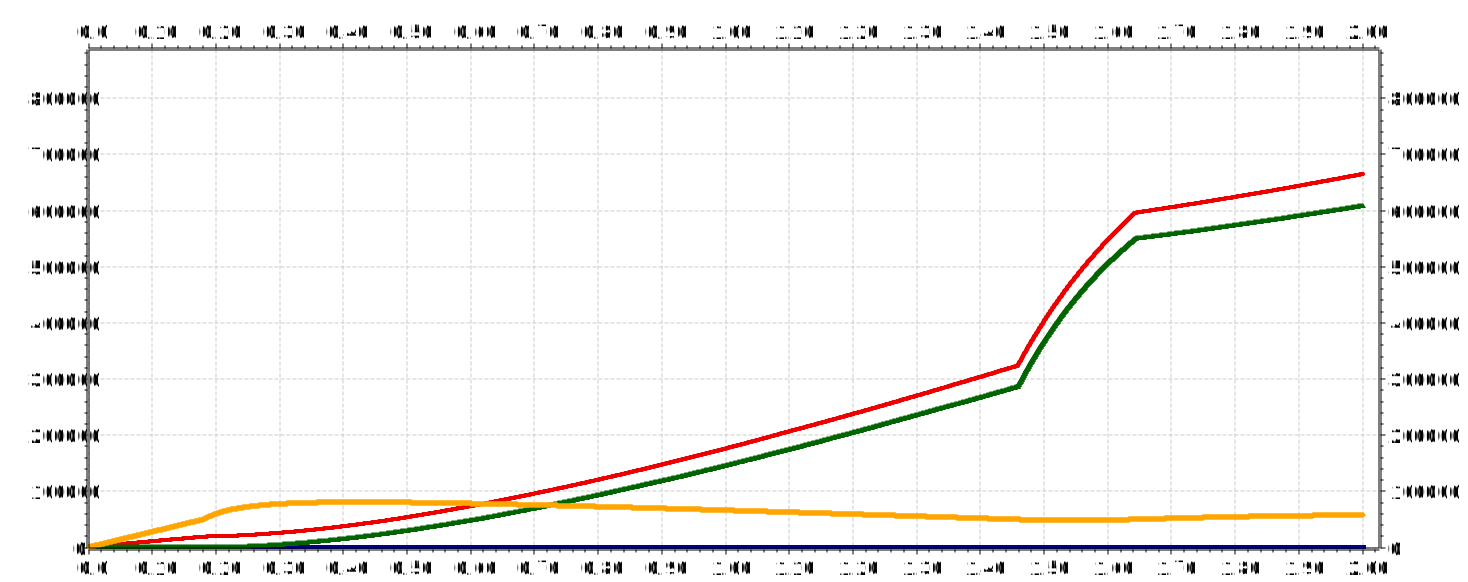
\includegraphics[width=\textwidth]{images/cexp_003_1.png}
                    \caption{FLC-enhanced scheduler results}
                \end{figure}

                \begin{figure}[!h]
                    \centering
                    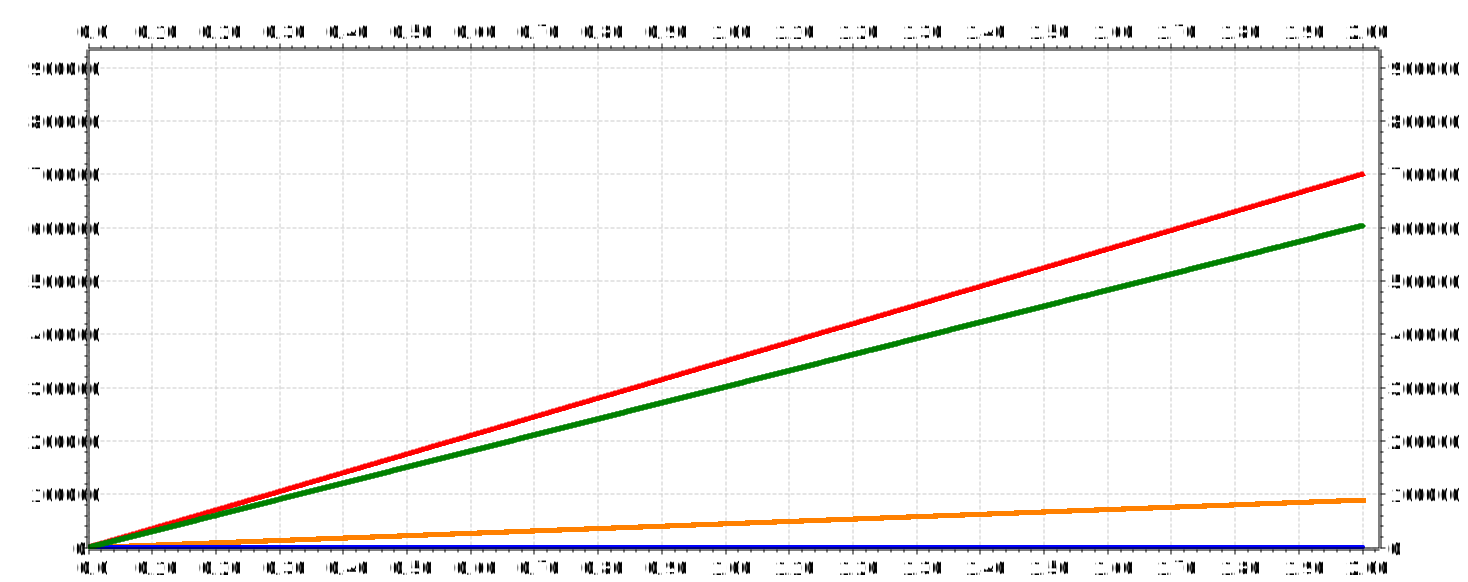
\includegraphics[width=\textwidth]{images/cexp_003_2.png}
                    \caption{Regular WRR scheduler results}
                \end{figure}
                \pagebreak

                In this experiment, I have prolonged the simulation time to 2 seconds, to get a better look at the convergence of the average delay in the FLC-enhanced case.

                Here, we notice that the FLC-enhanced scheduler is again superior to the regular scheduler, as the average delay of the real-time high-priority users converges to the desired value, while in the regular scheduler case this value rises slowly.

                Moreover, we no longer notice the compromise seen in the previous experiment, as even the lower priority user's average delays is slightly lower in the FLC-enhanced case than in the regular case. We may conclude that when there is more activity in a given priority class (be it because of more packets being generated or because of more users participating in the given class), the FLC-enhanced scheduler proves superior, with slight compromises being made depending on the situation at hand.

    \section{General conclusions}
    Given the presented experiments, we may conclude that the scheduler which features the FLC-enhancement is superior, under some circumstances, to the regular Weighted Round Robin scheduler. These circumstances include a higher network load and a higher high-priority population.

    It should be mentioned that these results apply to a chosen priority class (in this case, real-time high-priority), while the other classes are forced to compromise, to a certain degree. The magnitude of this compromise depends heavily on the situation at hand, but in general, if out goal is to be able to control the connection speed of a particular priority class, an FLC-enhanced scheduler is preferable.

    It might be interesting to experiment with the situation in which all the priority classes of a system are controlled by an FLC, with the average delays of each class being dynamically controlled, depending on the values of various network parameters, such as load, latency or per-class population.

    \pagebreak
    \section{References}
    \begin{enumerate}[label=(\arabic*)]
        \item{\verb|http://staff.cs.upt.ro/~todinca/cad/IP_scheduling.html|}
        \item{\verb|http://staff.cs.upt.ro/~todinca/TPAC/tpac.html|}
        \item{\verb|http://staff.cs.upt.ro/~todinca/FLA/FLA.html|}
        \item{\verb|https://doc.omnetpp.org/omnetpp/manual/|}
        \item{\verb|https://docs.omnetpp.org/tutorials/tictoc/|}
        \item{\verb|https://doc.omnetpp.org/omnetpp/api/|}
    \end{enumerate}
\end{document}